\section{Experiments}
    
    \frame{\sectionpage}

    \subsection{Experiment 1: Black vs White Experimenter}
    
    \begin{frame}{Experiment 1: Method}
        \begin{itemize}
            \item \underline{\textit{Participants}}: 7 men and 26 women
            \item \underline{\textit{Measure of automatic racial prejudice}}: IAT (how efficiently participants can pair Black/White names with positive/negative words)
            %\begin{itemize}
            %    \item prejudice-congruent associations are executed more efficiently 
            %    \item reveal not-consciously-endorsed or not-consciously-desire-to-be-endorsed associations
            %    \item unreliably correlated with denotatively related explicit attitudes
            %\end{itemize}
            \item \underline{\textit{Task awareness}}: participants were told that the procedure assesses prejudice
            \item \underline{\textit{Two phases}}
            \begin{itemize}
                \item prejudice congruent: mark \underline{Black-name negative-word} associations %and \underline{White-name positive-word} associations
                \item prejudice incongrent: mark \underline{Black-name positive-word} associations%and \underline{White-name-negative-word} associations
            \end{itemize}
            \item \underline{\textit{Variation}}: \underline{Black} versus \underline{White} experimenter
        \end{itemize}
    \end{frame}

    \begin{frame}{Experiment 1: Results}
        \begin{columns}

            \begin{column}{0.6\textwidth}
                \begin{figure}\label{fig:res1}
                \centering
                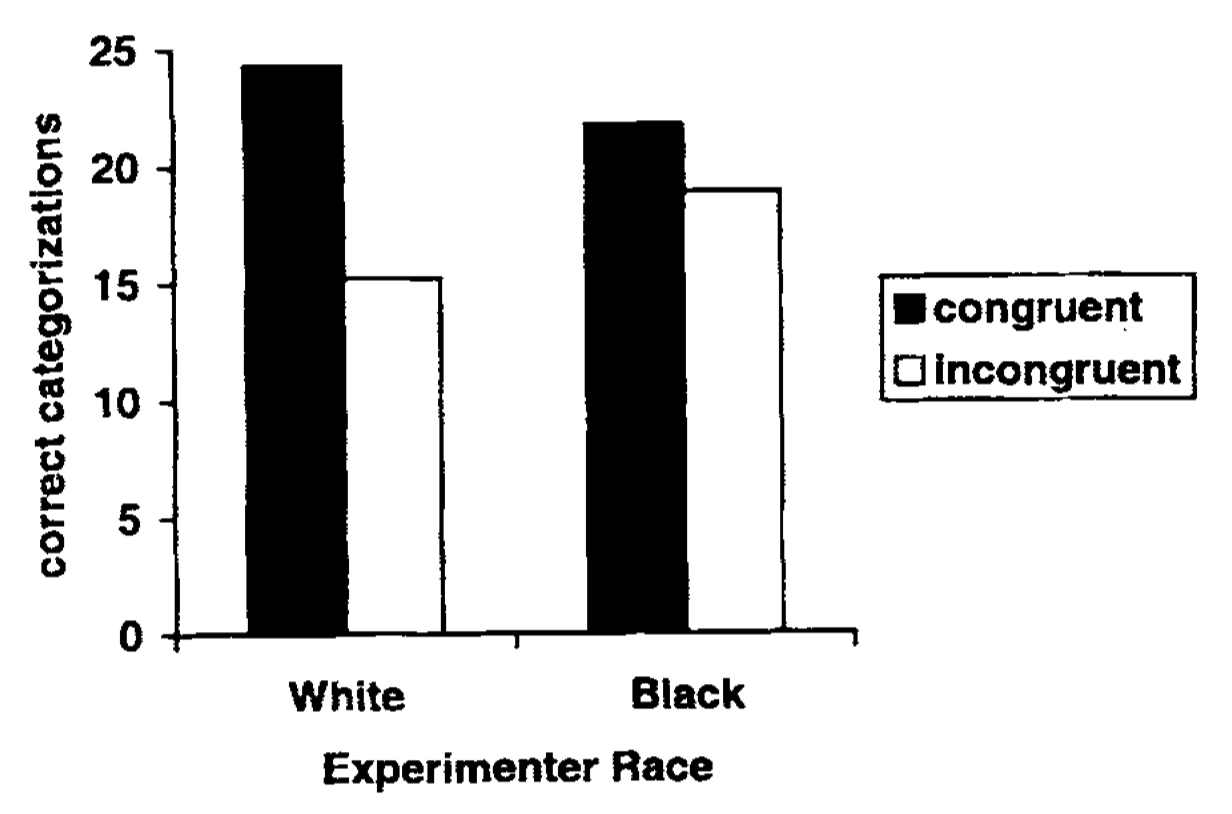
\includegraphics[height = 0.65 \textheight]{images/result1.png}
                \end{figure}
            \end{column}
            
            \begin{column}{0.4\textwidth}
        
            \only<2->{
                \small
                \begin{itemize}
                    \item<2-> more automatic anti-Black prejudice in the presence of a \underline{\textit{White}} experimenter
                    \item<3-> driven by more \underline{\textit{incongruent}} items categorized, \textcolor{lightlavender!55!white}{\textbf{NOT}} by less \underline{\textit{congruent}} items cateogrized
                \end{itemize}
                }
            % if stereotype activation is inevitable on exposure, more automatic anti-Black prejudice should be observed in the presence of a Black experimenter
            \uncover<4->{\textcolor{lightlavender!55!white}{\textbf{\underline{Question}}}: positive \textit{subtype}?}
            \end{column}
        \end{columns}
    \end{frame}

    \subsection{Experiment 2: Asian-American vs European-American participants}
    \begin{frame}{Shared Reality Theory}

        Social cooperation requires the establishment of \underline{\textit{shared understandings}} on dimensions relevant to the relationship.
        
        \uncover<2->{
            \vspace*{10pt}
            \textcolor{lightlavender!55!white}{\textbf{Relationship-specificity conjecture}}: automatic social tunning might be reduced/eliminated among participants who feel \textit{\underline{relatively invulnerable}} to the charge of anti-Black racism
        }

        \uncover<3->{
            \vspace*{10pt}
            \textcolor{lightlavender!55!white}{\textbf{Prediction}}
            \begin{itemize}
                \item Asian Americans exhibit \textit{\underline{less}} automatic social tuning
                \item subtype: equivalent effects
            \end{itemize}
        }
        

    \end{frame}

    \begin{frame}{Experiment 2: Method}
        \begin{itemize}
            \item \underline{\textit{Pilot}}: Sampled Asian Americans and European Americans are equivalently knowledgeable of African Americans
            \item \underline{\textit{Pre-experiment survey}}: explicit race-related attitudes
            \begin{itemize}
                \item Modern Racism Scale \citep[\textcolor{lightlavender!55!white}{\textbf{MRS}};][]{mcconahay1981has}
                \item Social Dominance Orientation Scale \citep[\textcolor{lightlavender!55!white}{\textbf{SDO}};][]{pratto1994social}
                \item Internal/External Motivation to Respond without Prejudice scales \citep[\textcolor{lightlavender!55!white}{\textbf{IMS,EMS}};][]{plant1998internal}
            \end{itemize} 
            \item \underline{\textit{Participants}}: 133 European American and 140 Asian American
            
        \end{itemize}
    \end{frame}

    \begin{frame}{Experiment 2: Results}
        \begin{columns}

            \begin{column}{0.45\textwidth}
                \begin{figure}
                \centering
                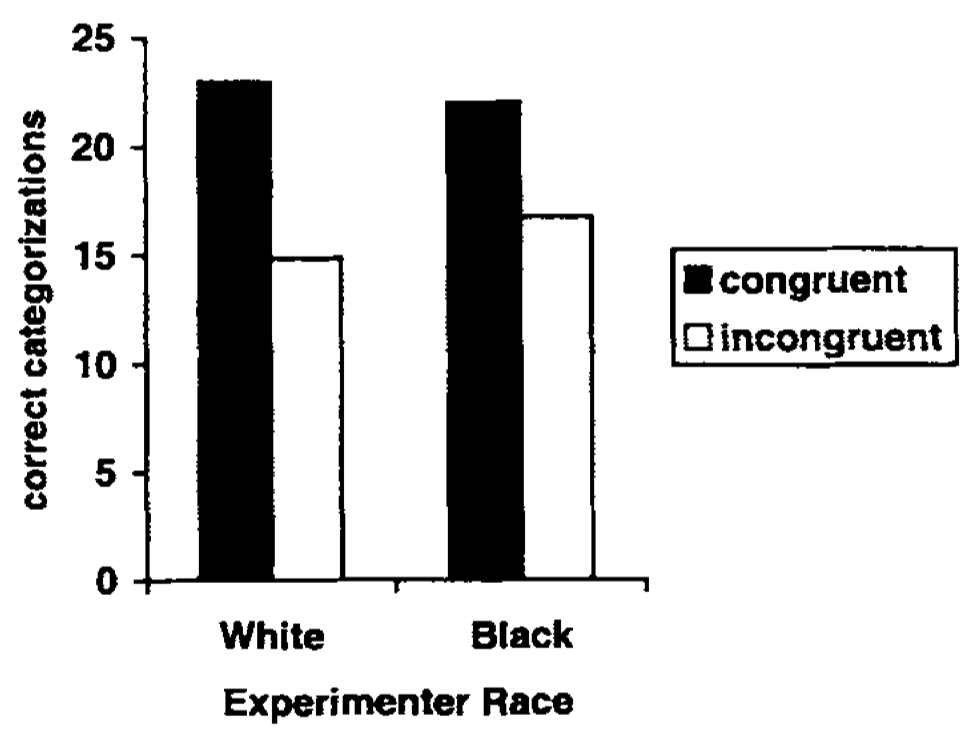
\includegraphics[height = 0.53 \textheight]{images/result2_euro.png}
                
                {\footnotesize European American Participants}
                \end{figure}
            \end{column}
            
            \begin{column}{0.45\textwidth}
                \begin{figure}
                    \centering
                    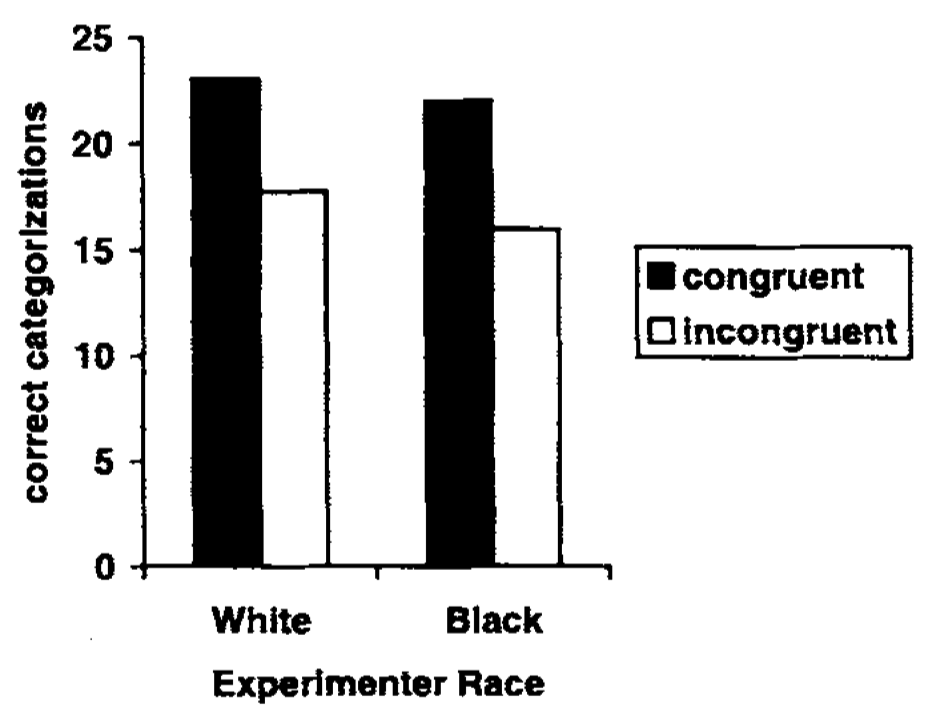
\includegraphics[height = 0.53 \textheight]{images/result2_asia.png}
                    
                    {\footnotesize Asian American Participants}
                \end{figure}
            \end{column}
        \end{columns}
        \vspace*{10pt}
        {\small Experimenter race affected the automatic prejudice of European American participants, but \textcolor{lightlavender!55!white}{\textbf{not}} Asian American participants.}
    \end{frame}

    \begin{frame}{Experiment 2: The Role of Explicit Attitudes}
        \begin{columns}

            \begin{column}{0.55\textwidth}
                \begin{table}[ht]
                    \footnotesize
                    \begin{center}
                      \begin{tabular}{lccccc}
                        
                        Measure & IAT & EMS & IMS & MRS & SDO  \\
                        \hline
                        IAT & - & \\
                        EMS & 0.03 & - \\
                        IMS & -0.01 & 0.06 & -\\
                        MRS & 0.03 & 0.19 & -0.38$^*$ & - \\
                        SDO & 0.09 & 0.15 & -0.35$^*$ & 0.56$^*$ & -
                      \end{tabular}
                    \end{center}
                  \end{table}
            \end{column}
            
            \begin{column}{0.4\textwidth}
                Some takeaways
                \begin{itemize}
                    \footnotesize 
                    \item IMS: European Americans are \textcolor{lightlavender!55!white}{\textbf{more}} internally motivated to respond without prejudice 
                    \item MRS: European Americans are \textcolor{lightlavender!55!white}{\textbf{less}} willing to express explicitly racist attitudes 
                    \item EMS: European Americans and Asian Americans are \textcolor{lightlavender!55!white}{\textbf{equally}} externally motivated to respond without prejudice
                \end{itemize}
            \end{column}
        \end{columns}
    \end{frame}

    \begin{frame}{Summary of Experiment 1 and 2}
    \begin{itemize}
        \item<+-> Results:
        \begin{itemize}
            \item \textit{\underline{Experiment 1}}: European Americans exhibited \textcolor{lightlavender!55!white}{\textbf{less automatic prejudice}} in the presence of a Black experimenter 
            \item \textit{\underline{Experiment 2}}: Asian Aemrican participants were \textcolor{lightlavender!55!white}{\textbf{unaffected}} by the experimenter race manipulation
        \end{itemize} 
        \item<+-> Consistency with shared reality theory
        \begin{itemize}
            \item Asian Americans expressed \textcolor{lightlavender!55!white}{\textbf{less}} explicit concern about their personal anti-Black prejudice
            \item \textbf{BUT}, no evidence that \textcolor{lightlavender!55!white}{\textbf{motivation to control prejudice}} accounts for participant ethnicity differences in automatic social tuning 
        \end{itemize}
        \item<+-> Further validate shared reality theory: manipulate the relationship with the Black experimenter
    \end{itemize}
    \end{frame}

    \subsection{Experiment 3: Asking Participants Not to Be Prejudiced vs. NOT Asking}
    
    \begin{frame}{Experiment 3: Method}
        \begin{itemize}
            \item \underline{\textit{Variation}}: the relevance of racial prejudice to participants' relationship with the experimenter
            \begin{itemize}
                \item attitude relevance moderating social tuning: \textcolor{lightlavender!55!white}{\textbf{equivalent levels of social tunning}} for European Americans and Asian Americans 
                \item subtyping: \textcolor{lightlavender!55!white}{\textbf{no impact}} on levels of automatic prejudice
                %\item also testing the impact of conscious goals on inhibiting the automatic activation of attitudes
            \end{itemize}
            \item \underline{\textit{Participants}}: 86 European American and 71 Asian American
            \item All experimenters were Black
            \item<+-> \underline{\textit{Explicit}} social influence: instructing participants to avoid prejudice
            
        \end{itemize}
    \end{frame}

    \begin{frame}{Experiment 3: Results}
        \begin{columns}

            \begin{column}{0.45\textwidth}
                \begin{figure}
                \centering
                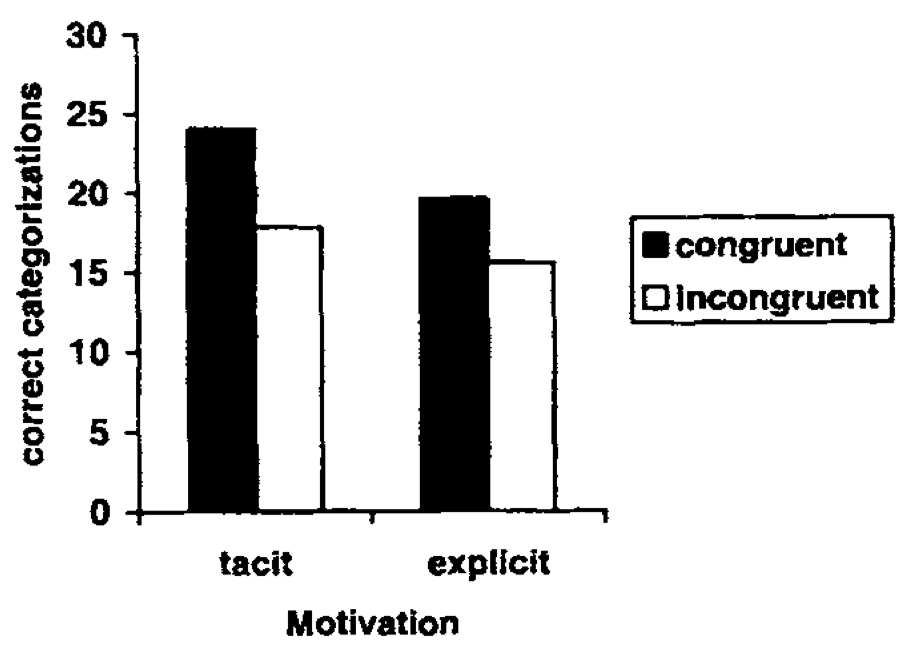
\includegraphics[height = 0.48 \textheight]{images/result3_euro.png}
                
                {\footnotesize European American Participants}
                \end{figure}
            \end{column}
            
            \begin{column}{0.45\textwidth}
                \begin{figure}
                    \centering
                    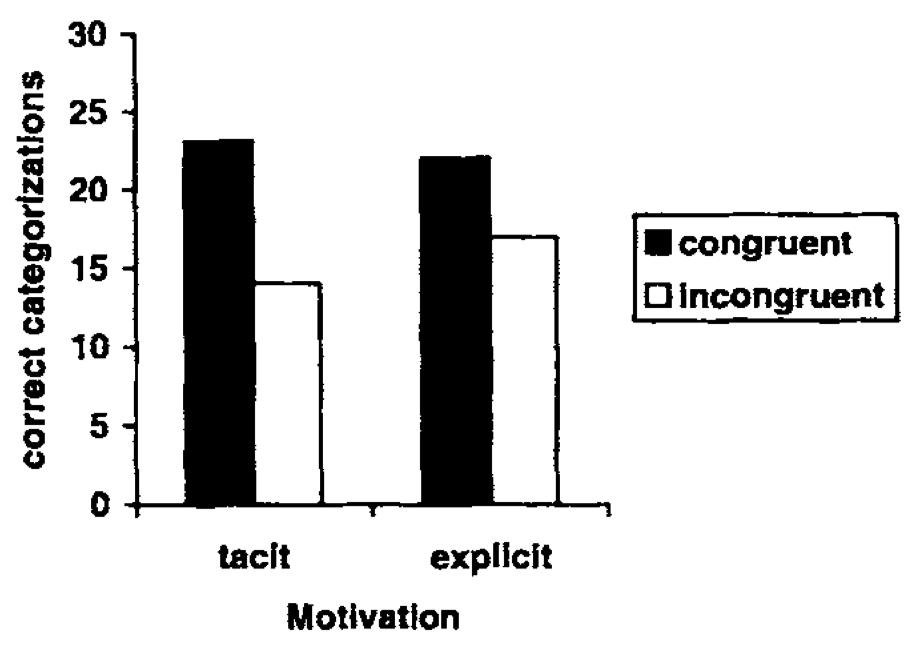
\includegraphics[height = 0.48 \textheight]{images/result3_asia.png}
                    
                    {\footnotesize Asian American Participants}
                \end{figure}
            \end{column}
        \end{columns}
        \vspace*{10pt}
        {\small \textcolor{lightlavender!55!white}{\textbf{Both}} European American and Asian American participants exhibited \textcolor{lightlavender!55!white}{\textbf{equivalent}} automatic social tuning as a function of \textit{\underline{explicit}}} social influence, while \textcolor{lightlavender!55!white}{\textbf{unable}} to deliberately manipulate IAT performance
    % A fundamental challenge to current understandings of automaticity (\textit{back then}), a conscious goal evokes an automatic process that competes withe activation of automatic prejudice, it's possible that conscious intent might reduce the level of automatic prejudice expressed
    \end{frame}

    \subsection{Experiment 4: Subliminal Priming Procedure}
    \begin{frame}{Experiment 4: The Validity of IAT}
        Using a subliminal priming procedure to assess automatic racial prejudice {\footnotesize \citep{bargh1996automaticity,chen1997nonconscious,lepore1997category,wittenbrink2001spontaneous}}
        \begin{itemize}
            \item flashes of White and Black faces, followed by either \textit{good}, or \textit{bad}
            \item prejudice measure
            \begin{itemize}
                \item anti-Black prejudice: the degree to which responses are quicker to \textit{bad} than \textit{good} after exposure to Black faces
                \item pro-White prejudice: the degree to which responses are quicker to \textit{good} than \textit{bad} after exposure to Black faces
            \end{itemize}
        \end{itemize}
    \end{frame}
    
    \begin{frame}{Experiment 4: Replicating Experiment 1}
        
        \begin{columns}
            \begin{column}{0.45\textwidth}
                \begin{figure}
                \centering
                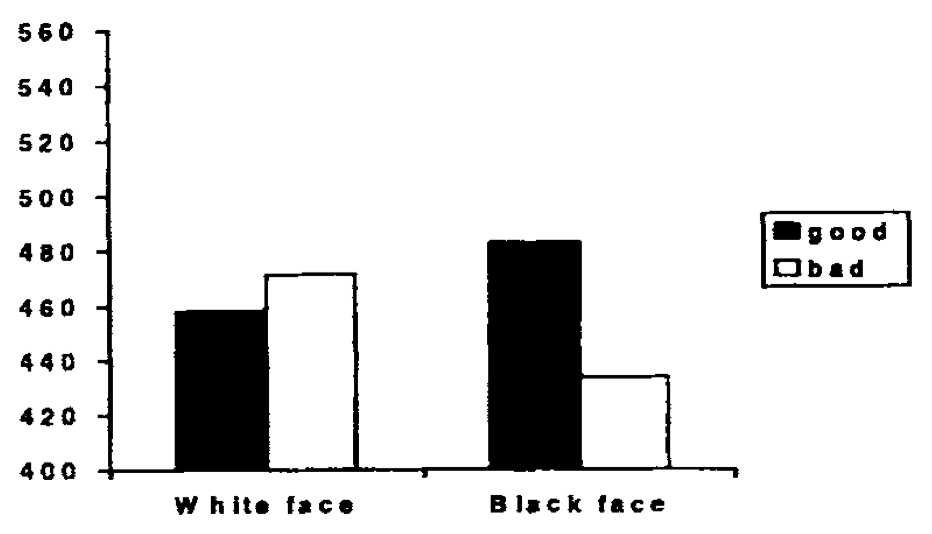
\includegraphics[height = 0.43 \textheight]{images/result4_1_white.png}
                
                {\footnotesize White Experimenter}
                \end{figure}
            \end{column}
            
            \begin{column}{0.45\textwidth}
                \begin{figure}
                    \centering
                    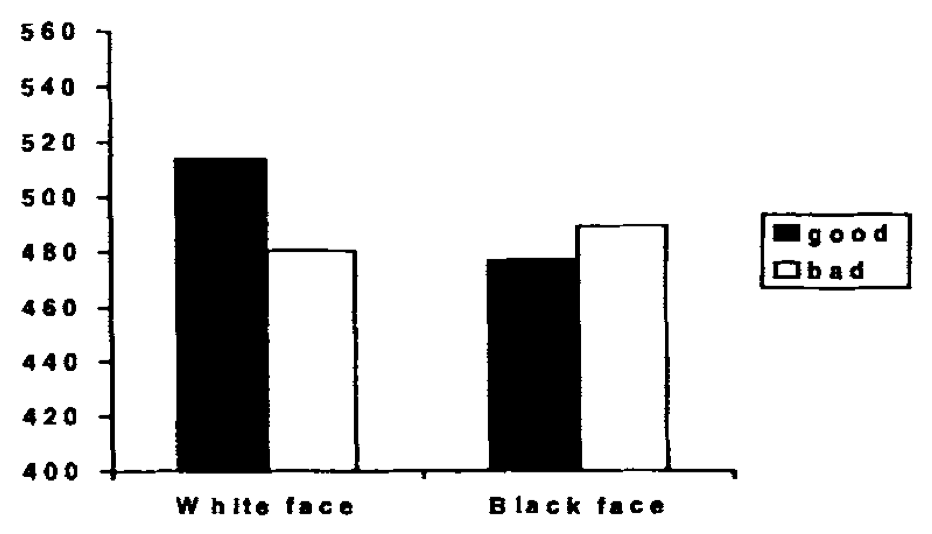
\includegraphics[height = 0.43 \textheight]{images/result4_1_black.png}
                    
                    {\footnotesize Black Experimenter}
                \end{figure}
            \end{column}
        \end{columns}
        \vspace*{10pt}
        European Americans exhibited \textcolor{lightlavender!55!white}{\textbf{less automatic prejudice}} in the presence of a Black experimenter \textcolor{lightlavender!55!white}{$\checkmark$}
    \end{frame}

    \begin{frame}{Experiment 4: Replicating Experiment 2}
        
        \begin{columns}
            \begin{column}{0.45\textwidth}
                \begin{figure}
                \centering
                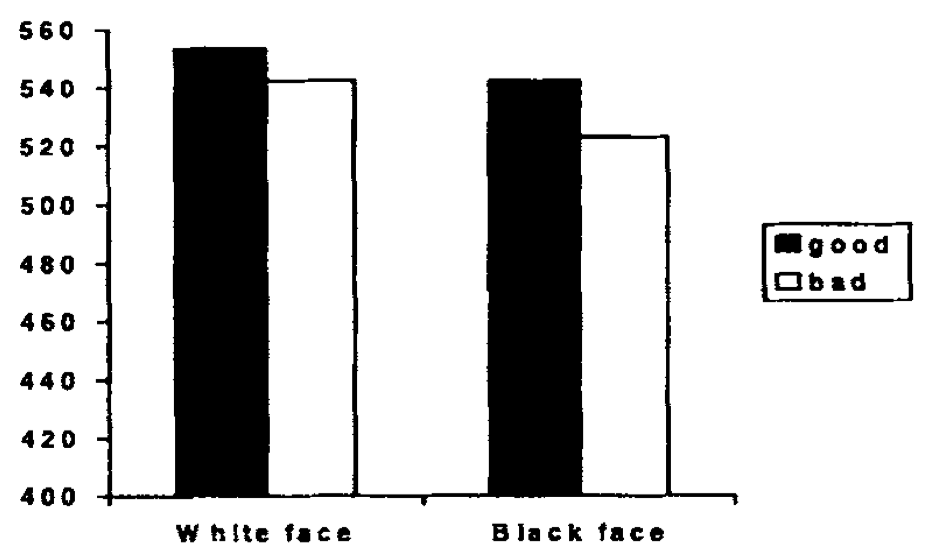
\includegraphics[height = 0.43 \textheight]{images/result4_2_white.png}
                
                {\footnotesize White Experimenter}
                \end{figure}
            \end{column}
            
            \begin{column}{0.45\textwidth}
                \begin{figure}
                    \centering
                    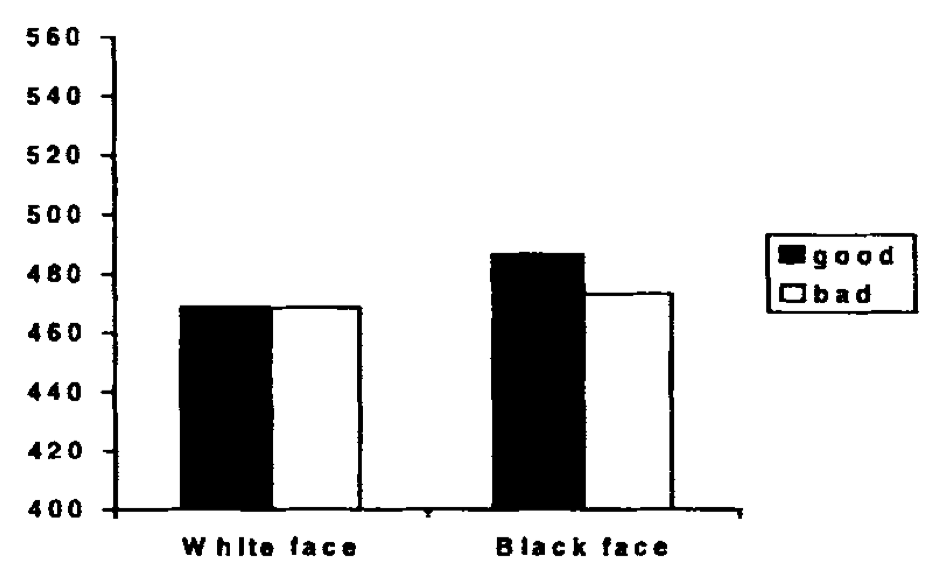
\includegraphics[height = 0.43 \textheight]{images/result4_2_black.png}
                    
                    {\footnotesize Black Experimenter}
                \end{figure}
            \end{column}
        \end{columns}
        \vspace*{10pt}
        Asian Americans' \textcolor{lightlavender!55!white}{\textbf{automatic prejudice}} is unaffected the race of the experimenter \textcolor{lightlavender!55!white}{$\checkmark$}
    \end{frame}